% !TeX root = probability.tex

%%%%%%%%%%%%%%%%%%%%%%%%%%%%%%%%%%%%%%%%%%%%%%%%%%%%%%%%%%%%%%

\section{קיץ תש"פ מועד ב}

\begin{center}
\selectlanguage{english}
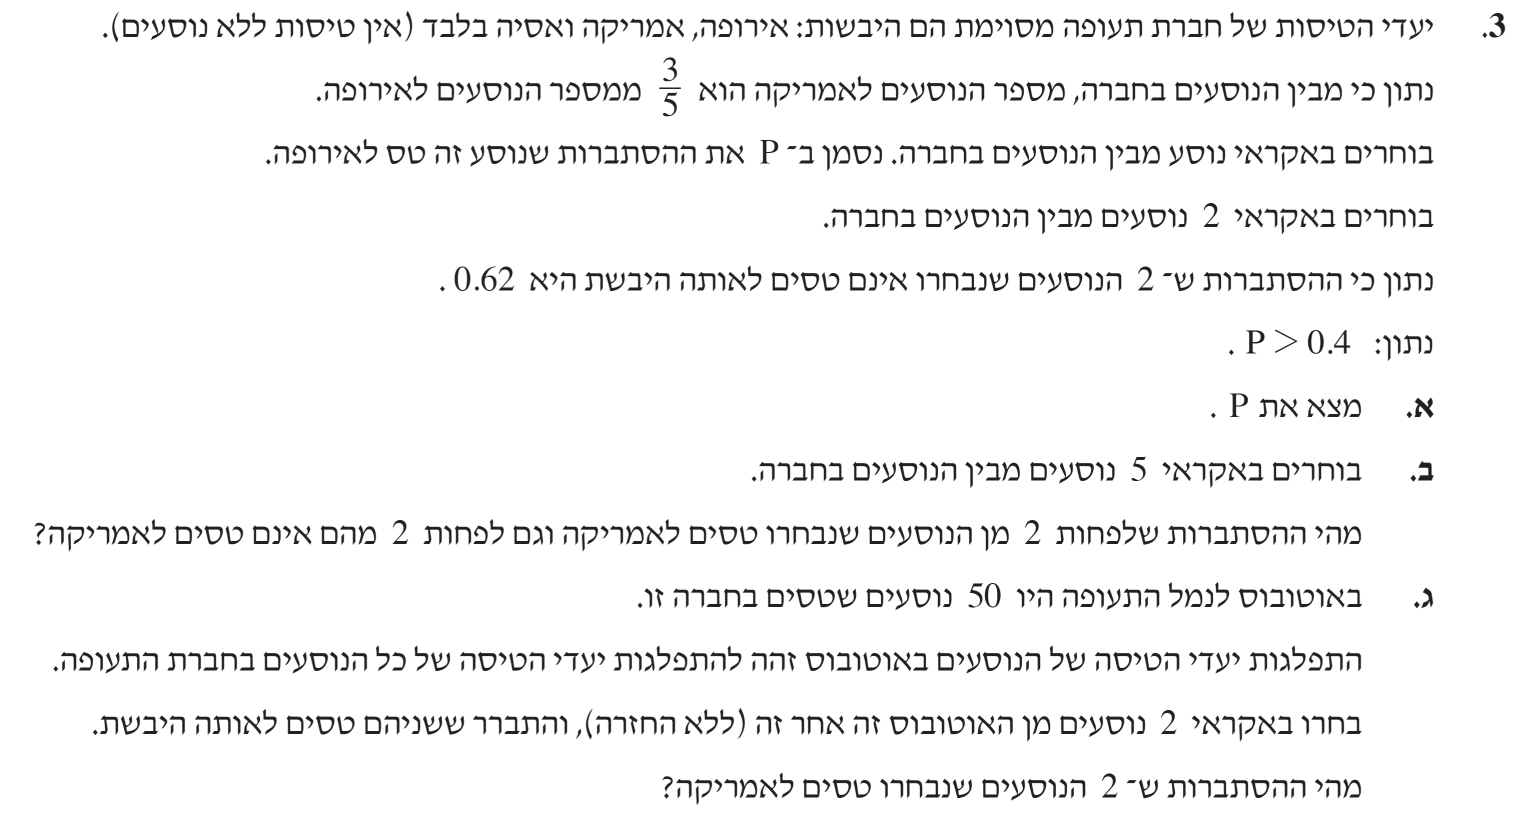
\includegraphics[width=.85\textwidth]{summer-2020b-3}
\end{center}

נסמן את המאורעות:
$AM$ 
עבור טיסה לאמריקה,
$EU$
עבור טיסה לאירופה,
$AS$
עבור טיסה לאסיה. נתון
$P(EU)=p$.\footnote{%
אני מעדיף אות קטנה 
$p$
עבור ההסתברות כי אות גדולה תמיד מסמנת את ההסתברות של מאורע כגון
$P(EU)$.}
לפי המידע הנתון
$P(AM)=\frac{3}{5}p$
ולפי הסתברות משלימה
$P(AS)=1-p-\frac{3}{5}p=1-\frac{8}{5}p$.

\textbf{סעיף א}

נניח שהבחירות של שני הנוסעים של יעדי הטיסות בלתי-תלויות. נתון שההסתברות שבחרו בטיסות שונות היא 
$0.62$.
אפשר לחשב הסתברות זו אבל אפשר גם לחשב את ההסתברות המשלימה
$0.38$
ששניהם בחרו את אותו יעד:
\begin{eqn}
p^2 + \left(\frac{3}{5}p\right)^2+\left(1-\frac{8}{5}p\right)^2&=&0.38\\
p^2 + \frac{9}{25}p^2+1-\frac{16}{5}p+\frac{64}{25}p^2&=&0.38\\
98p^2 -80p+15.5 &=&0\,.
\end{eqn}
נפתור את המשוואה הריבועית ונקבל
$p=\frac{80\pm 18}{196}= 0.5, 0.3$.
השאלה מבקשת הסתברות גדול מ-%
$0.4$
ולכן התשובה היא
$0.5$.

\textbf{סעיף ב}

נסמן את ההסתברות המבוקשת ב-%
$AM22$.
הדרך היחידה שגם לפחות שניים טסים לאמריקה ושניים לא היא ששלושה טסים לשם ושניים לא, או להיפך. ההסתברות לטיסה לאמריקה היא
$\frac{3}{5}p=0.3$.
לפי חוק ברנולי:
\[
P(AM22)={5 \choose 2}(0.3)^2(0.7)^3 +{5 \choose 2}(0.7)^2(0.3)^3=
(10\cdot 0.09 \cdot 0.49) (0.7+0.3)=0.441\,.
\]

\begin{center}
\begin{tikzpicture}
[grow=right,
level 1/.append style={level distance=4cm,
                       sibling distance=7em},
level 2/.append style={level distance=4cm,
                       sibling distance=2.5em}]
\node[left] {$\scriptstyle (15,25,10)$} % root
child {
  node[right] {$\scriptstyle (15,25,9)$}
    child {
      node[right] {$\scriptstyle AS2$}
      edge from parent node[below] {$\scriptstyle 9/49$}
    }
    child {
%      node[right] {$$}
      edge from parent 
        node[below,near end] {$\scriptstyle 25/49$}
    }
    child {
%      node[right] {$$}
      edge from parent node[above] {$\scriptstyle 15/49$}
    }
    edge from
      parent node[below,yshift=-2mm] {$\scriptstyle 10/50$}
      node[above right] {\R{אסיה}}
}
child {
  node[right] {$\scriptstyle (15,24,10)$}
    child {
%      node[right] {$$}
      edge from parent node[below] {$\scriptstyle 10/49$}
    }
    child {
      node[right] {$\scriptstyle EU2$}
      edge from parent 
      node[below,near end] {$\scriptstyle 24/49$}
    }
    child {
%      node[right] {$$}
      edge from parent node[above] {$\scriptstyle 15/49$}
    }
    edge from parent node[below] {$\scriptstyle 25/50$}
      node[above] {\R{אירופה}}
}
child {
  node[right] {$\scriptstyle (14,25,10)$}
    child {
%      node[right] {$$}
      edge from parent node[below] {$\scriptstyle 10/49$}
    }
    child {
%      node[right] {}
      edge from parent 
        node[below,near end] {$\scriptstyle 25/49$}
    }
    child {
      node[right] {$\scriptstyle AM2$}
      edge from parent node[above] {$\scriptstyle 14/49$}
    }
    edge from parent
      node[above,yshift=2mm] {$\scriptstyle 15/50$}
      node[below right] {\R{אמריקה}}
}
;
\end{tikzpicture}
\end{center}

\textbf{סעיף ג}

אני נפלתי בפח כאן ולא הבנתי שהניסוח "ששניהם" ו-"שני הנוסעים שנבחרו" מכוון להסתברות מותנית. ניסוח מקובל יותר היה "שניים מבין הנוסעים שטסים לאותו יבשת טסים לאמריקה.

בחרו שני נוסעים אחד לאחר השני ללא החזרה, ולכן יש לארגן את המידע בעץ. כאשר 
$AM2, EU2, AS2$
מסמנים את המאורעות ששני נוסעים טסים לאותו יבשת, ו-%
$Y2AM2\cup EU2 \cup AS2$
מסמן ששני נוסעים טסים ליבשת כלשהי.  נשתמש בעובדה ש-%
$AM2 \subseteq Y2)$.
ונחשב את הסתברות המבוקשת:
\begin{eqn}
P(AM2/Y2)&=&
\frac{P(AM2 \cap Y2)}{P(Y2)}=\frac{P(AM2)}{P(Y2)}\\[12pt]
&=&\frac{\frac{15}{50}\cdot \frac{14}{49}}
{\frac{15}{50}\frac{14}{49}+\frac{25}{50}\frac{24}{49}+
\frac{10}{50}\frac{9}{49}}\\[12pt]
&=&\frac{15\cdot 14}{15\cdot 14+25\cdot 24+10\cdot 9}\\[12pt]
&=& \frac{21}{90}=\frac{7}{30}\,.
\end{eqn}


%%%%%%%%%%%%%%%%%%%%%%%%%%%%%%%%%%%%%%%%%%%%%%%%%%%%%%%%%%%%%

\section{קיץ תש"פ מועד א}

\begin{center}
\selectlanguage{english}
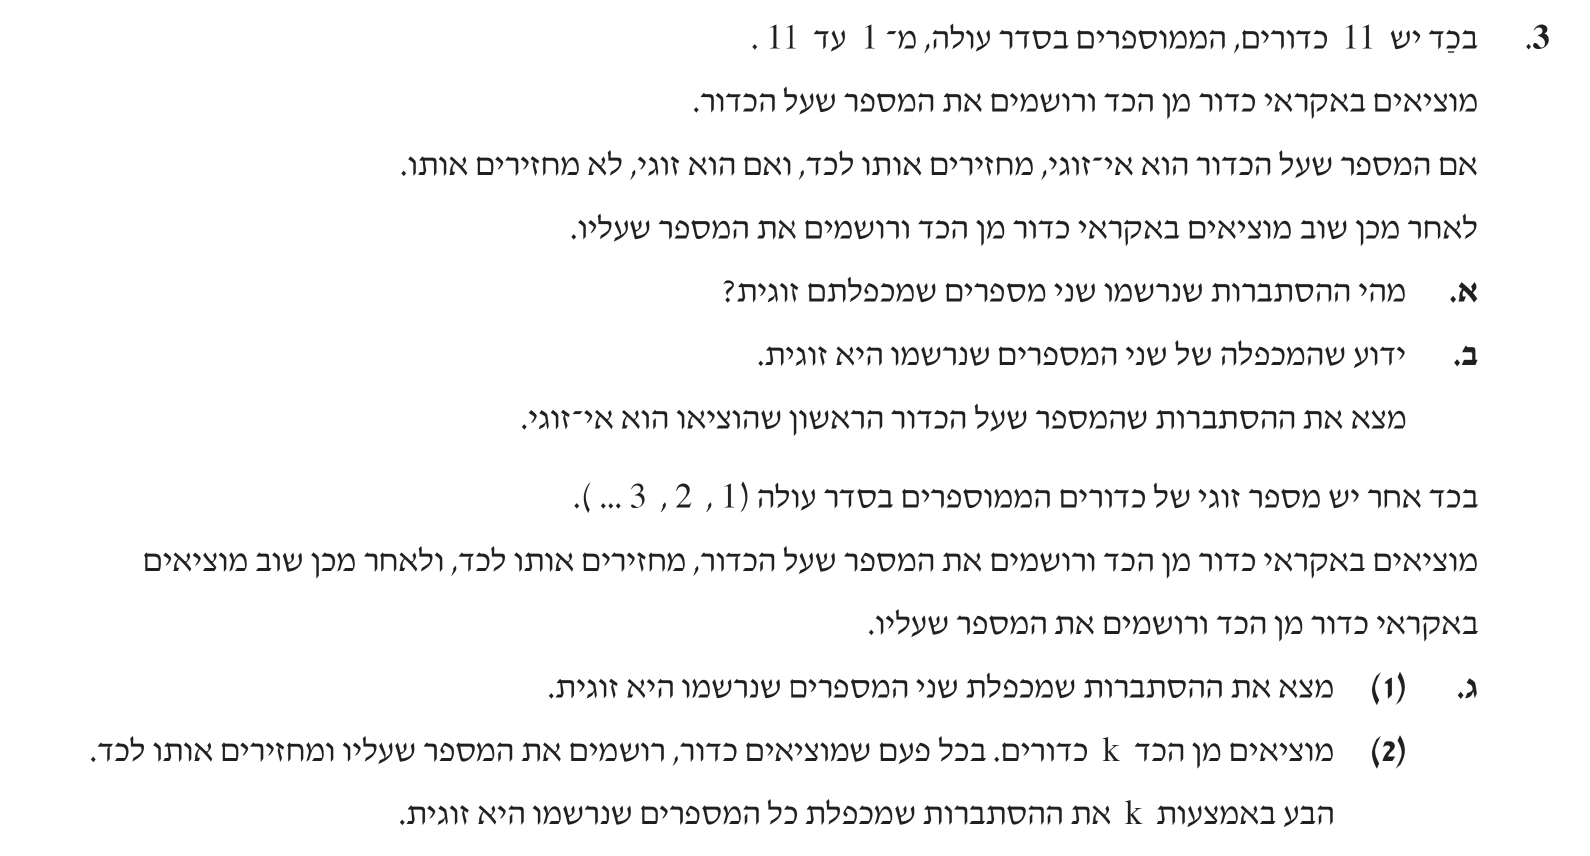
\includegraphics[width=.9\textwidth]{summer-2020a-3}
\end{center}

\textbf{סעיף א}

נסמן ב-%
$Z1,Z2$
את המאורעות של לשליפת כדור עם מספר זוגי בשליפה הראשונה והשנייה, נסמן ב-%
$I1,I2$
את המאורע של שליפת כדור אי-זוגי בשליפה הראשונה והשנייה ונסמן ב-%
$MZ$
את המאורע שהמכפלה של שני המספרים זוגית. מכפלה של שני מספרים שלמים היא זוגית אלא שניהם אי-זוגיים
$2k\cdot n = 2kn$
מספר זוגי ללא קשר לערך של 
$n$
אבל
$(2k+1)(2n+1)= 4kn + 2k + 2n +1$
הוא מספר אי-זוגי. השליפה של כדורים עם מספרים אי-זוגיים היא עם החזרה ולכן:
\[
P(MZ)=1-P(I1)P(I2)=1-\frac{6}{11}\cdot \frac{6}{11}=\frac{85}{121}\,.
\]

\textbf{סעיף ב}

המילה "ידוע" מכוון להסתברות מותנית. כדי להמכפלה תהיה זוגית כאשר המספר הראשון הוא אי-זוגי, השני חייב להיות זוגי. שוב נזכור שיש החזרה לאחר שליפת כדור עם מספר אי-זוגי ונקבל:
\[
P(I1/MZ) = \frac{P(I1\cap MZ)}{P(MZ)}= \frac{P(I1)P(Z2)}{P(MZ)}=
\frac{\frac{6}{11}\cdot\frac{5}{11}}{\frac{85}{121}}=\frac{6}{17}\,.
\]
שימו לב שלא השתמשנו בנתון שאין החזרה של שליפה של כדור עם מספר זוגי.

\textbf{סעיף ג 1}

בכד יש מספר שווה של כדורים עם מספרים זוגיים ועם אי-זוגיים ולכן ההסתברות לשלוף כדור עם מכפלה אי-זוגי היא 
$1-P(I1)P(I2)=1-\frac{1}{2}\cdot\frac{1}{2}=\frac{3}{4}$.

\textbf{סעיף ג 2}

מכפלת כל המספרים זוגית אלא אם כל 
$k$
המספרים הם אי-זוגיים, ולכן:
\[
P(MZ)=1-\left(\frac{1}{2}\right)^k\,.
\]

%%%%%%%%%%%%%%%%%%%%%%%%%%%%%%%%%%%%%%%%%%%%%%%%%%%%%%%%%

\section{חורף תש"פ}

\begin{center}
\selectlanguage{english}
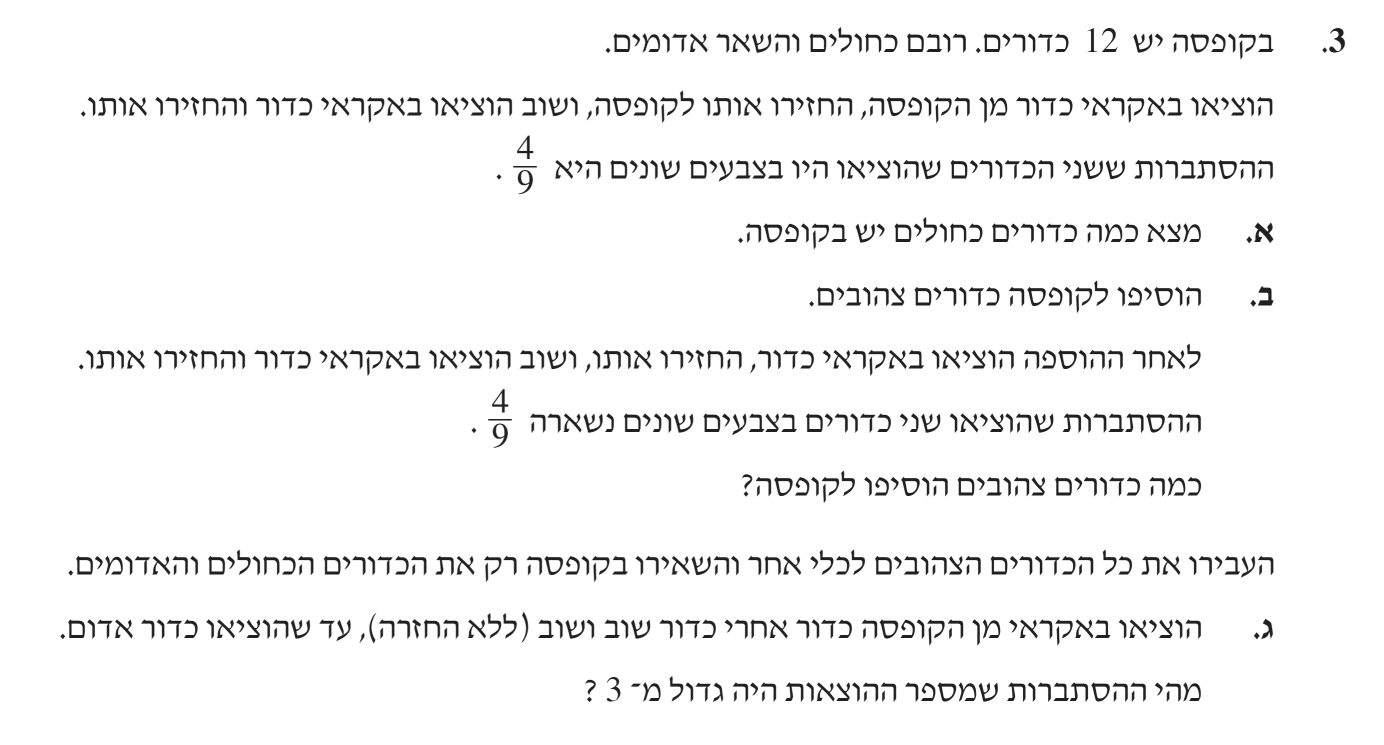
\includegraphics[width=.85\textwidth]{winter-2020-3}
\end{center}

\textbf{סעיף א}

נסמן ב-%
$K$ \L{(kahol)}
את המאורע של שליפת כדור כחול, נסמן ב-%
$A$ \L{(adom)}
את המאורע של שליפת כדור אדום ונסמן ב-%
$S$ \L{(shonim}
את המאורע של שליפת שני כדורים בצבעים שונים. שתי שליפות בלתי-תוליות של כדורים מכוון לעץ הסתברויות אבל המקרה כאן פשוט ונתקדם ישר לנוסחה. השליפה היא עם החזרה ולכן 
$P(KA)=P(AK)$
ההסתברות המבוקשת היא:
\begin{eqn}
P(S) &=& P(KA) + P(AK) = 2P(KA) = 2\left(\frac{K}{12}\cdot \frac{A}{12}\right)=\frac{4}{9}\\
18KA &=& 4\cdot 144\\
KA &=& 32\,.
\end{eqn}
בהתחשב באילוצים
$K+A=12, K>A$
הפתרון היחיד הוא
$K=8,A=4$.

\textbf{סעיף ב}

נסמן ב-%
$T$ \L{(tzahov)}
את המאורע של שליפת כדור צהוב. כמו בסעיף הקודם 
$P(KA)=P(AK)$, $P(KT)=P(TK)$, $P(AT)=P(TA)$.
ההסתברות המבוקשת היא:
\begin{eqn}
P(S) &=& 2(P(KA)+P(KT)+P(AT))=\frac{4}{9}\\
&=&2\left(\frac{32}{(12+T)^2}+\frac{8T}{(12+T)^2}+\frac{4T}{(12+T)^2}\right)=\frac{4}{9}\\
54T+144 &=& T^2 + 24T + 144\\
T&=&30\,.
\end{eqn}
$T=0$
הוא פתרון כי ברור שההסתברות לא משתנה אבל נניח שאכן מוסיפים מספר חיובי של כדורים.
\begin{center}
\begin{tikzpicture}
  [grow=right,
   level 1/.append style=
     {level distance=6em,sibling distance=4em},
   level 2/.append style=
     {level distance=6em,sibling distance=4em},
   level 3/.append style=
     {level distance=6em,sibling distance=4em}
  ]
  \node[left] {$(8,4)$}
    child {node[right]  {$(8,3)$}
        edge from parent node [below] {\R{אדום}} 
    }
    child {node [right] {$(7,4)$}
      child {node[right]  {$(7,3)$} 
          edge from parent node [below] {\R{אדום}}
      } 
      child {node[right]  {$(6,4)$}
        child {node[right]  {$(6,3)$}
            edge from parent node [below] {\R{אדום}}
        }
        child {node[right] {$(5,4)$}
            edge from parent node [above] {\R{כחול}}
        }
        edge from parent node [above] {\R{כחול}}
      }
      edge from parent node [above] {\R{כחול}}
    };
\end{tikzpicture}
\end{center}

\textbf{סעיף ג}

חזרנו למצב הראשון עם שמונה כדורים כחולים וארבעה אדומים. הדרך הקצרה לחשב את ההסתברות המבוקשת היא לחשב את ההסתברות המשלימה לשליפת כדור אדום בשליפה הראשונה, השנייה או השלישית. השליפה היא ללא החזרה ולכן ההסתברויות תלויות. ניתן לארגן את המידע בעץ (למעלה) כאשר בכל צומת רשום
$(K,A)$.
נסמן ב-%
$P(AR)$ \L{(adom rishon)}
את השליפה של הכדור האדום הראשון. ההסתברות המבוקשת היא:
\begin{eqn}
P(AR) &=& 1-\left[P(A) + P(K)P(A) + P(K)P(K)P(A)\right]\\[6pt]
&=& 1-\left[\frac{4}{12} + \frac{8}{12}\cdot\frac{4}{11} +
   \frac{8}{12}\cdot\frac{7}{11}\cdot\frac{4}{10}\right]\\[6pt]
&=&1-\frac{984}{1320}=\frac{14}{55}\,.
\end{eqn}
